\newpage
\noindent
\begin{minipage}{\textwidth}
  \textbf{\sffamily\Huge Pedo[Arte]Metria}
\end{minipage}\\
\begin{figure*}[ht!]
  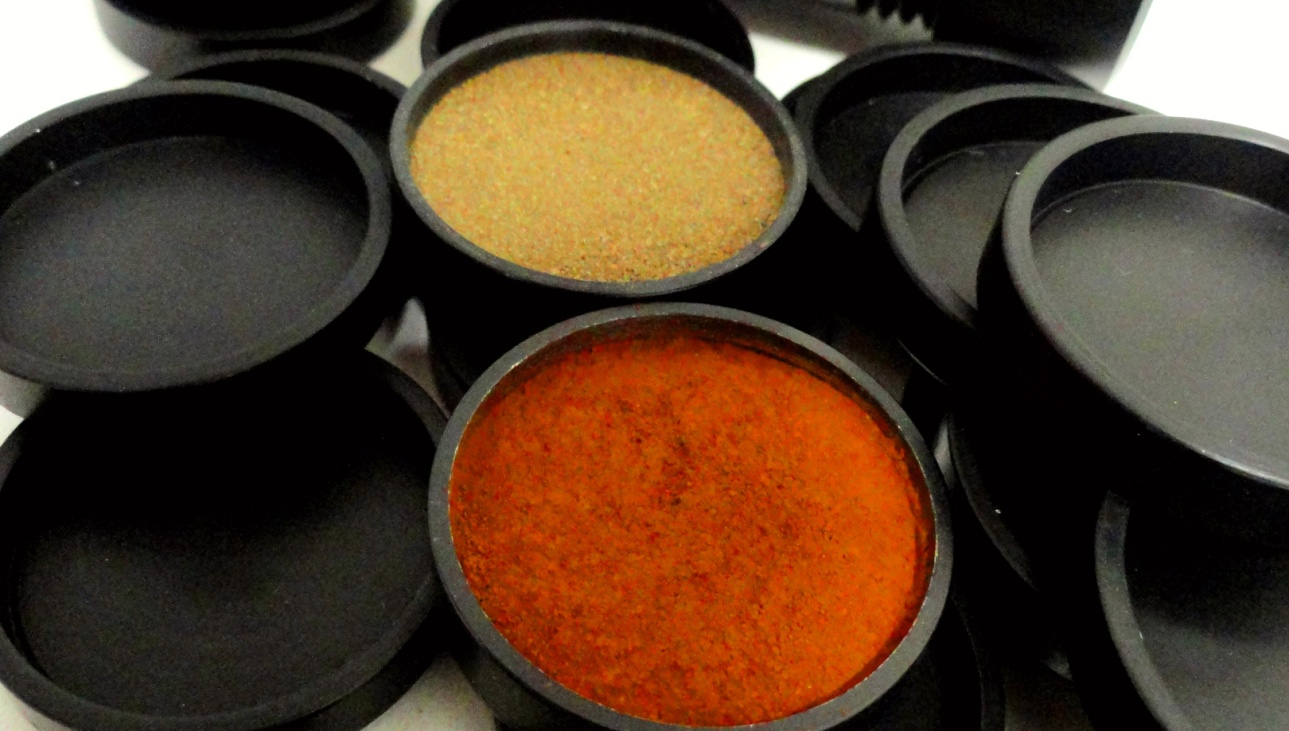
\includegraphics[width=\textwidth]{figuras/pedoartemetria}
\end{figure*}\\
\vspace*{0.5cm}\\
\raggedleft
\begin{minipage}{0.8\textwidth}
  \raggedleft
  \LARGE
  \noindent\textbf{A cor do solo}\\
  \vspace*{0.5cm}\\
  \noindent{Para um olhar desavisado, não se trata de maquiagem. São porta amostras para avaliação da espectroscopia de refletância difusa, uma das técnicas mais indicadas para quantificar os óxidos de ferro (hematita e gohetita) como alternativa a técnica convencional de difração de Raio-X.}\\
  \vspace*{0.5cm}\\
  \normalsize{\noindent\textit{Foto enviada por: Diego Silva Siqueira -- Grupo de Pesquisa CSME da UNESP Campus de Jaboticabal}}\\
\end{minipage}
\vfill
\raggedright
\begin{minipage}{0.5\textwidth}
  \rule{\textwidth}{1mm}\\
  \normalsize
  Se você quer compartilhar conosco uma imagem \textbf{\sffamily Pedo[Arte]Métrica} de sua autoria, envie-a para \href{mailto:pedometria.news@gmail.com}{pedometria.news@gmail.com} com resolução de 300 dpi ou com no mínimo 5Mb, preferencialmente em formato PNG.
\end{minipage}}